% TODO L10 Open-Source Software

\ifuniversity{tubs}{\date{June 23, 2025}}

\author{Thomas Thüm}
\lecture{Open-Source Software}{opensource}

\section{Open-Source Software}
\subsection{Open-Source Development}
\begin{frame}{\insertsubsection\ \mytitlesource{\sommerville}} % copied from se1
	\begin{fancycolumns}
		\begin{definition}{Open-Source Development}
			\mycite{\emph{Open-source development} is an approach to software development in which the source code of a software system is published and volunteers are invited to participate in the development process.} % Raymond 2001
		\end{definition}
		\begin{note}{Open-Source Development}
			\begin{itemize}
				\setlength\itemsep{.0em}
				\item assumption in the early days: code developed by small core group
				\item today: Internet to recruit volunteer developers (often users)
				\item volunteers contribute with bug reports, feature requests, changes to the software (cf.\ pull requests)
				\item core group controls changes to main repo
				\item opposite: proprietary software / closed-source development
			\end{itemize}
		\end{note}
		\nextcolumn
		\begin{note}{Internet iff Open Source}
			\begin{itemize}
				\setlength\itemsep{.0em}
				\item Internet used to distribute source code and recruit developers
				\item Internet builds on open-source software
			\end{itemize}
		\end{note}
		\begin{example}{Examples} % TODO separate slides with images?
			\begin{itemize}
				\setlength\itemsep{.0em}
				\item operating system Linux (for most servers)
				\item operating system Android (for most clients)
				\item web server Apache
				\item database management system mySQL
				\item browser Firefox
				% TODO \item e-mail client Thunderbird
				\item image editor GIMP
				\item media player VLC
				\item screen recording software OBS
				\item video editing software Shotcut
				\item runtime env.\ and standard library OpenJDK
				\item development environment Eclipse
			\end{itemize} % 
		\end{example}
	\end{fancycolumns}
\end{frame}

\subsection{Central Questions for Each Software Project}
\begin{frame}{\insertsubsection\ \mytitlesource{\sommerville}} % copied from se1
	\begin{fancycolumns}
		\begin{note}{First Question}
			\mycite{Should the product that is being developed make use of open-source components?}
		\end{note}
		\begin{example}{Example Criteria}
			\begin{itemize}
				\item are related open-source components available?
				\item is their quality sufficient?
				\item will they be maintained?
				\item what is the effort to integrate them?
				\item is it cheaper to modify or redevelop them?
				\item how are they licensed?
			\end{itemize}
		\end{example}
		\nextcolumn
		\begin{note}{Second Question}
			\mycite{Should an open-source approach be used for its own software development?}
		\end{note}
		\begin{example}{Example Criteria}
			\begin{itemize}
				\item business model: how to earn money then? % TODO does not mean it is free
				\item support? consulting? proprietary extensions? -- \textit{rich relatives or friends? unconditional basic income \deutsch{bedingungsloses Grundeinkommen}?}
				\item what additional value do you have from opening the source?
				\item more customers, recognition, collaborations?
				\item does it reveal confidential business knowledge?
			\end{itemize}
		\end{example}
	\end{fancycolumns}
\end{frame}

\xkcdframe{1810} % chat clients

\subsection{Richard Stallman's Four Freedoms}
\begin{frame}{\insertsubsection\ \mytitlesource{\href{https://www.youtube.com/watch?v=Ag1AKIl_2GM}{Stallman's 2014 TEDx Talk}}}
	\begin{fancycolumns}
		\centering\pic[width=.6\linewidth,trim=0 0 0 0,clip]{people/richard-stallman}
		\vspace{-7mm}
		
		\begin{note}{}
			Richard Matthew Stallman aka.\ RMS (born 1953)
		\end{note}
		\nextcolumn
		\begin{definition}{Four Freedoms by Richard Stallman}
			\begin{itemize}
				\item 0. freedom to run it for whatever purpose
				\item 1. freedom to study and modify the program (source code is available)
				\item 2. freedom to redistribute it (needed for non-programmers)
				\item 3. freedom to redistribute or even sell modified versions
				\item all four needed that the user controls the program
				\item otherwise the program controls the users
			\end{itemize}
		\end{definition}
	\end{fancycolumns}
\end{frame}

\subsection{Free Software}
\begin{frame}{\insertsubsection\ \mytitlesource{\href{https://www.youtube.com/watch?v=Ag1AKIl_2GM}{Stallman's 2014 TEDx Talk}}}
	\begin{fancycolumns}
		\begin{definition}{Free Software}
			\begin{itemize}
				\item free stands for freedom (often confused with \mycite{free of charge})
				\item free software: demand for freedom
				\item open-source software: better code quality (promoted by Eric S.\ Raymond)
				\item today largely replaced with term open-source software
				\item more inclusive term?\\free and open-source software (FOSS) % TODO wikipedia defines this term to be the subset of both worlds https://en.wikipedia.org/wiki/Free_and_open-source_software
			\end{itemize}
		\end{definition}
		\begin{note}{Free Software vs Freeware}
			\begin{itemize}
				\item free software: free as in free speech
				\item freeware: free as in free beer
			\end{itemize}
			free software can be adware or shareware
		\end{note}
		\nextcolumn
		\begin{definition}{Free Software Foundation \mysource{\href{https://www.fsf.org/}{fsf.org}}}
			\begin{itemize}
				\item founded by Richard Stallman in 1985
				\item first ten years: employ developers for the operating system GNU
				
				Linux = GNU + Linux kernel
				\item later: promoting free software, working on legal issues
			\end{itemize}
		\end{definition}
		\begin{exampletight}{}
			\centering\pic[width=.5\linewidth]{opensource/gnu-logo}
		\end{exampletight}
	\end{fancycolumns}
\end{frame}

\subsection{Buying Free Software}
\begin{frame}{\insertsubsection}
	\begin{fancycolumns}
		\centering\pic[height=65mm,trim=0 500 0 600,clip]{opensource/buying-free-software-gimp}
		\nextcolumn
		\centering\pic[height=65mm,trim=0 500 0 600,clip]{opensource/buying-free-software-vlc}
	\end{fancycolumns}
\end{frame}

\lessonslearned{
	\item Open-source development and open-source software
	\item Examples and central questions around open source
	\item Free software foundation: four freedoms, RMS, FOSS
	\item Next: What are main principles of open-source software?
}{
	\item \sommerville\mychapter{7.4} Open-Source Development
	\item \href{https://www.youtube.com/watch?v=Ag1AKIl_2GM}{Stallman's 2014 TEDx Talk}
%\href{https://www.ulm.ccc.de/ccc/chaosseminar/2004_11_gefahren_der_softwarepatente/}{Stallman's lecture in Ulm}
}{
	\begin{enumerate}
		\item Form groups of 2--3 students
		\item Which open-source software are you using?
		\item Have you ever made use of the four freedoms?
	\end{enumerate}
}

\section{Open-Source Principles}
\subsection{Rights and Duties}
\begin{frame}{\insertsubsection} % copied from se1
	\begin{fancycolumns}
		\begin{definition}{Who owns the code? \mysource{\sommerville}}
			\mycite{Although a fundamental principle of open-source development is that source code should be freely available, this does not mean that anyone can do as they wish with that code. Legally, the developer of the code (either a company or an individual) owns the code. They can place restrictions on how it is used by including legally binding conditions in an \emph{open-source software license}.} % St. Laurent 2004
		\end{definition}
		\begin{note}{What if there is no license?}
			\begin{itemize}
				\item you are allowed to read the code
				\item you are \emph{not allowed} to use, modify, distribute it
				\item you need to contact the owners to negotiate
			\end{itemize}
		\end{note}
		\nextcolumn
		\begin{definition}{Understanding Software Licenses \mysource{\href{https://fossa.com/blog/open-source-licenses-101-mit-license/}{fossa.com}}}
			\mycite{Anyone who works with open-source software (OSS), whether as a developer, a contributor, or a business, has to know at least a little bit about open source licenses. In a nutshell, an open source license tells you what you can and can’t do with the open source code. And if using the code comes with any requirements and/or responsibilities, the license outlines those as well.}
		\end{definition}
		\begin{example}{What's Next?}
			\begin{itemize}
				\item principles of software licenses
				\item examples of famous software licenses
			\end{itemize}
		\end{example}
	\end{fancycolumns}
\end{frame}

\subsection{Collective Ownership}
\begin{frame}{\insertsubsection}
	\begin{fancycolumns}
		\centering\pic[width=\linewidth,trim=800 0 100 0,clip]{people/sercan-leylek}
		\vspace{-7mm}
		
		\begin{note}{Sercan Leylek (2016) \mysource{\href{https://storksnestblog.wordpress.com/2016/10/19/every-programmer-is-an-author/}{wordpress.com}}}
			\mycite{Every programmer is an author.}
		\end{note}
		% author, programmer, blogger
		\nextcolumn
		\begin{note}{Mosher’s Law of Software Engineering \mysource{\href{https://twitter.com/codewisdom/status/777924969221226501}{twitter.com}}}
			\mycite{Don’t worry if it doesn’t work right. If everything did, you’d be out of a job.}
		\end{note}
		% TODO find out who Mosher is/was
	\end{fancycolumns}
\end{frame}

\widexkcdframe{306} % orphaned projects % copied from se1

\subsection{Recommendations for Companies}
\begin{frame}{\insertsubsection} % copied from se1
	\begin{fancycolumns}
		\begin{note}{Motivation}
			\begin{itemize}
				\item basically every company needs software
				\item even non-software companies need software
				\item more and more companies even transition into software companies (e.g., car manufacturers)
				\item large amounts of money spend on software licenses (e.g., Microsoft Windows and Office, Adobe Acrobat)
				\item even if open-source software is for free, resources are necessary to prevent license violations within a company
				\item and who does the maintenance? who pays for it?
			\end{itemize}
		\end{note}
		\nextcolumn
		\begin{definition}{Bayersdorfer 2007: \mysource{\sommerville}}
			\begin{itemize}
				\item track information about downloaded and used open-source components (e.g., storing licenses)
				\item understand how a component is licensed before it is used
				\item study the open-source project to predict its future evolution
				\item educate developers about open source and open-source licensing \correct
				\item auditing of open-source software to detect violations
				\item if you rely on open-source products, support their development
			\end{itemize}
		\end{definition}
	\end{fancycolumns}
\end{frame}

\subsection{Copyleft and Copyright}
\begin{frame}{\insertsubsection} % copied from se1
	\begin{fancycolumns}[reverse,T]
		\begin{definition}{{Copyleft \hfill\tikz[overlay] \node[anchor=-10,xshift=2mm] {\pic[width=.13\linewidth]{opensource/copyleft}};}}
			\begin{itemize}
				\item right to freely distribute and modify intellectual property
				\item obligation that the same rights (license) apply to derivative work
				\begin{itemize}
					\item \emph{weak copyleft}: only applies to formerly-licensed parts (e.g., a library)
					\item \emph{strong copyleft}: applies to the complete software (deprecatory: viral effect)
				\end{itemize}
				\item license without copyleft is called \emph{permissive}
				\item implemented with copyright laws
			\end{itemize}
		\end{definition}
		\begin{example}{Examples for Copyleft Licenses}
			\small
			\begin{itemize}
				\item GNU General Public License (GPL) for software
				\item Creative Commons share-alike license for documents and pictures
			\end{itemize}
		\end{example}
		\nextcolumn
		\begin{definition}{{\tikz[overlay] \node[anchor=190,xshift=-2mm] {\pic[width=.13\linewidth]{opensource/copyright}};\hfill Copyright \deutsch{Urheberrecht}}}
			\begin{itemize}
				\item kind of intellectual property, such as patents and trademarks \deutsch{gestiges Eigentum, Patent, Marke}
				\item owner of creative work has exclusive right over copies for a limited time
				\item includes distribution, reproduction, public performance, derivative work
				\item copyright is often granted by national laws
			\end{itemize}
		\end{definition}
		\begin{note}{Decision for copyleft is independent of:}
			\begin{itemize}
				\item decision to allow/forbid commercial use
				\item decision about the fee to get the source code
			\end{itemize}
		\end{note}
	\end{fancycolumns}
\end{frame}

\subsection{The Impact of Licensing Issues}
\begin{frame}{\insertsubsection\ \mytitlesource{\href{https://www.heise.de/news/Ruby-on-Rails-Durch-Lizenzproblem-entfallene-Library-erzeugt-Dominoeffekt-5999197.html}{heise.de}}} % copied from se1
	\begin{fancycolumns}
		\begin{exampletight}{}
			\pic[width=\linewidth]{opensource/heise-ruby-on-rails-license-problem} % TODO in German. translate? replace?
		\end{exampletight}
		\nextcolumn
		\begin{example}{March 2021: The Story of mimemagic}
			\begin{itemize}
				\item Ruby library mimemagic is part of Ruby on Rails and was licensed under MIT license
				\item 580,000 repositories on Github use Ruby on Rails under the same license
				\item mimemagic is using another library under GPL license
				\item GPL has a copyleft: mimemagic must be published under GPL too
				\item old versions of mimemagic have been removed
				\item new versions use GPL license
				\item 580,000 projects would need to change from MIT to GPL and upgrade to the new version
			\end{itemize}
		\end{example}
	\end{fancycolumns}
\end{frame}


\lessonslearned{
	\item Need for and impact of software licenses
	\item Ownership and code without any license
	\item Recommendations for companies
	\item Copyleft and its impact on software
	\item Next: What are major licenses?
}{
	\item \sommerville\mychapter{7.4} Open-Source Development
}{
	\begin{enumerate}
		\item Form groups of 2--3 students
		\item Does published code without a license fulfill the four freedoms?
		\item What is the problem of creating a license for every project?
	\end{enumerate}
}

\section{Open-Source Licenses}
\subsection{MIT License}
\begin{frame}{\insertsubsection\ \mytitlesource{\href{https://fossa.com/blog/open-source-licenses-101-mit-license/}{fossa.com}}} % copied from se1
	\begin{fancycolumns}
		\begin{definition}{Profile}
			\begin{itemize}
				\item released: about 1987
				\item publisher: Massachusetts Institute of Technology
				\item classification: permissive
				\item most popular license % TODO provide evidence https://en.wikipedia.org/wiki/MIT_License
				\item prominent use: Ruby on Rails (server-side web application framework), Node.js (JavaScript runtime environment)
			\end{itemize}
		\end{definition}
		\begin{example}{Selected Terms and Conditions}
			\begin{itemize}
				\item permits reuse within proprietary software
				\item license shipped with distribution or relicensing (even to proprietary licenses)
				\item \mycite{provided as-is, without warranty}
			\end{itemize}
		\end{example}
		\nextcolumn
		\begin{exampletight}{}
			\centering\pic[width=.55\linewidth]{opensource/mit-logo}
		\end{exampletight}
		\begin{note}{The Full License Text}
			\tiny\mycite{Copyright (c) \textless year\textgreater \textless copyright holders\textgreater
				
				Permission is hereby granted, free of charge, to any person obtaining a copy of this software and associated documentation files (the "Software"), to deal in the Software without restriction, including without limitation the rights to use, copy, modify, merge, publish, distribute, sublicense, and/or sell copies of the Software, and to permit persons to whom the Software is furnished to do so, subject to the following conditions:
				
				The above copyright notice and this permission notice shall be included in all copies or substantial portions of the Software.
				
				THE SOFTWARE IS PROVIDED "AS IS", WITHOUT WARRANTY OF ANY KIND, EXPRESS OR IMPLIED, INCLUDING BUT NOT LIMITED TO THE WARRANTIES OF MERCHANTABILITY, FITNESS FOR A PARTICULAR PURPOSE AND NONINFRINGEMENT. IN NO EVENT SHALL THE AUTHORS OR COPYRIGHT HOLDERS BE LIABLE FOR ANY CLAIM, DAMAGES OR OTHER LIABILITY, WHETHER IN AN ACTION OF CONTRACT, TORT OR OTHERWISE, ARISING FROM, OUT OF OR IN CONNECTION WITH THE SOFTWARE OR THE USE OR OTHER DEALINGS IN THE SOFTWARE.}
		\end{note}
	\end{fancycolumns}
\end{frame}

\subsection{GPL: GNU General Public License}
\begin{frame}{\insertsubsection\ \mytitlesource{\href{https://www.gnu.org/licenses/gpl-3.0.html}{gnu.org}}} % copied from se1
	\begin{fancycolumns}
		\begin{definition}{Profile}
			\begin{itemize}
				\setlength\itemsep{.0em}
				\item releases: 1989 (GPLv1), 1991 (GPLv2), 2007 (GPLv3)
				\item author/publisher: Richard Stallman, Free Software Foundation
				\item classification: strong copyleft
				\item prominent use: Linux kernel (GPL-2.0-only), GNU Compiler Collection (GCC)
			\end{itemize}
		\end{definition}
		\begin{example}{Selected Terms and Conditions}
			\begin{itemize}
				\setlength\itemsep{.0em}
				\item software using (modified) GPL software must be released under GPL (copyleft) % TODO find better formulation
				\item for any sale or distribution: binaries must be accompanied by source code
				\item for private/interal use: no obligations
				\item commercial redistribution allowed
				\item GPL software (Linux/GCC) may be used for commercial purposes
			\end{itemize}
		\end{example}
		\nextcolumn
		\begin{exampletight}{}
			\centering\pic[width=.55\linewidth]{opensource/gplv3-logo}
		\end{exampletight}
		\begin{note}{Three Main Versions}
			\begin{itemize}
				\item GPL-1.0-only and GPL-1.0-or-later
				\begin{itemize}
					\item publishing binary only was allowed
					\item applies to whole distributable
				\end{itemize}
				\item GPL-2.0-only and GPL-2.0-or-later
				\begin{itemize}
					\item fixed above problems
					\item relaxed version LGPL, motivated by C standard library (libc)
				\end{itemize}
				\item GPL-3.0-only and GPL-3.0-or-later
				\begin{itemize}
					\item improved compatibility with other licenses (e.g., Apache)
				\end{itemize}
			\end{itemize}
		\end{note}
	\end{fancycolumns}
\end{frame}

\subsection{LGPL: GNU Lesser General Public License}
\begin{frame}{\insertsubsection\ \mytitlesource{\href{https://www.gnu.org/licenses/lgpl-3.0.html}{gnu.org}}} % copied from se1
	\begin{fancycolumns}
		\begin{definition}{Profile}
			\begin{itemize}
				\item releases: 1991 (LGPLv2), 1999 (LGPLv2.1), 2007 (LGPLv3)
				\item formerly known as: GNU Library General Public License
				\item publisher: Free Software Foundation
				\item classification: weak copyleft
				%\item prominent use: 
			\end{itemize}
		\end{definition}
		\begin{example}{Selected Terms and Conditions}
			\begin{itemize}
				\item similar to GPL, but less restrictive
				\item software using (modified) LGPL software components \emph{does not have to} be released under LGPL
				\item modifications of LGPL software components \emph{must} be released under LGPL % TODO does not have to be released!
				\item freedom only for LGPL components
			\end{itemize}
		\end{example}
		\nextcolumn
		\begin{exampletight}{}
			\centering\pic[width=.55\linewidth]{opensource/lgplv3-logo}
		\end{exampletight}
		\begin{note}{Three Main Versions}
			\begin{itemize}
				\item LGPL-2.0-only and LGPL-2.0-or-later
				%				\begin{itemize}
					%					\item publishing binary only was allowed
					%					\item applies to whole distributable
					%				\end{itemize}
				\item LGPL-2.1-only and LGPL-2.1-or-later
				%				\begin{itemize}
					%					\item fixed above problems
					%					\item relaxed version LGPL, motivated by C standard library (libc)
					%				\end{itemize}
				\item LGPL-3.0-only and LGPL-3.0-or-later
				%				\begin{itemize}
					%					\item improved compaitibility with other licenses (e.g., Apache)
					%				\end{itemize}
			\end{itemize}
		\end{note}
		\begin{example}{What's the main problem of LGPL?}
			\centering It contains \mycite{GPL}!\\[2mm]LGPL often confused with GPL in industry.
		\end{example}
	\end{fancycolumns}
\end{frame}

\xkcdframe{225}

\subsection{Compatibility of Software Licenses}
\begin{frame}{\insertsubsection}% TODO \ \mytitlesource{\href{}{}}}}
\begin{fancycolumns}
\begin{note}{Problem}
	\begin{itemize}
		\item most licenses have similar goals
		\item still: sometimes legally impossible to combine software with different licenses
		\item incompatibilities often arise from copyleft clauses
	\end{itemize}
\end{note}
\begin{example}{Desired Incompatibilities}
	\begin{itemize}
		\item proprietary licenses are typically specific to a program and incompatible to each other
		\item copyleft licenses are incompatible to proprietary and permissive licenses
		\item software licensed with \emph{GPL} cannot be used within \emph{MIT}-licensed software
	\end{itemize}
\end{example}
\nextcolumn
\begin{example}{Undesired Incompatibilities}
	\begin{itemize}
		\item software licensed with \emph{GPL-2.0-only} cannot be used within \emph{GPLv3}- or \emph{LGPLv3}-licensed software (cf.\ Linux kernel) $\Rightarrow$ most projects use \emph{GPL-2.0-or-later} instead
		\item software licensed with \emph{GPLv3} cannot be used in material licsensed as creative commons \emph{BY-SA 4.0} \mysource{\href{https://creativecommons.org/share-your-work/licensing-considerations/compatible-licenses/}{creativecommons.org}}
	\end{itemize}
\end{example}
\begin{exampletight}{Overview on Compatibilities}
	\centering\pic[width=\linewidth]{opensource/compatibility} % TODO nachzeichnen mit Tikz? oder ersetzen durch https://commons.wikimedia.org/wiki/File:Software_licensing_spectrum.png
\end{exampletight}
\end{fancycolumns}
\end{frame}
%     compatible: MIT->GPL
%     incompatible: GPL->MIT

\subsection{Re-Licensing and Dual Licensing}
\begin{frame}{\insertsubsection}
\begin{fancycolumns}
\begin{note}{How to solve a license incompatibility?}
	\begin{itemize}
		\item remove the software everywhere
		\item re-implement (parts thereof)
		\item give it a new license (as replacement or in addition to the old license)
	\end{itemize}
\end{note}
\begin{definition}{Re-Licensing}
	\begin{itemize}
		\item changing the license to another license
		\item requires consent by all developers
		\item in practice 100\% often not feasible: 80--95\%
	\end{itemize}
\end{definition}
\begin{example}{{Re-Licensing of the VLC Project\hfill\tikz[overlay] \node[anchor=30,xshift=2mm] {\pic[height=12mm]{opensource/vlc}};}} % TODO add references and double check years https://en.wikipedia.org/wiki/License_compatibility
	\begin{itemize}
		\item removed from the Apple App Store
		\item re-licensed from GPLv2 to LGPLv2
		\item later re-licensed to Mozilla Public License
	\end{itemize}
\end{example}
\nextcolumn
\begin{definition}{Dual Licensing}
	\begin{itemize}
		\item owner is not bound to the own copyleft/license
		\item a software can have multiple licenses
		\item same rules as for re-licensing
		\item term also used for 3 and more licenses
	\end{itemize}
\end{definition}
\pic[height=12mm]{opensource/netscape}\hfill\pic[height=12mm]{opensource/firefox}
\begin{example}{Mozilla's Firefox Browser} % TODO add references and double check years https://en.wikipedia.org/wiki/License_compatibility https://en.wikipedia.org/wiki/Software_relicensing
	\begin{itemize}
		\item Netscape's Communicator 4.0 released under the Mozilla Public License
		\item incompatilibility to GPL
		\item dual licensing as MPLv1.1/GPLv2/LGPLv2.1
	\end{itemize}
\end{example}
\end{fancycolumns}
\end{frame}

\lessonslearned{
	\item Software licenses: MIT, GPL, LGPL
	\item License incompatibilities: desired and undesired
	\item Re-licensing and dual licensing
	\item Next: How to systematically reuse software?
}{
	\item \sommerville\mychapter{7.4} Open-Source Development
}{
	Quiz in \StudIP

	~
	
	\centering\fancyqr{color=black,height=30mm}{https://studip.tu-braunschweig.de/dispatch.php/course/courseware/courseware/18333?cid=635f5186b364a369979d0f45ab2ace1d\#/structural\_element/421053}
}
% se1 interaction
%	\begin{enumerate}
%		\item Form groups of 2--3 students
%		\item Find three example for software systems were you would recommend any of the following licenses: MIT, GPL, LGPL
%		\item What are reasons for the license over the other two licenses?
%	\end{enumerate}

%\faq{
%	\item
%}{
%	\item
%}{
%	\item
%}

\input{../se1/template/footer}

% TODO L11 Software Product Lines

\ifuniversity{tubs}{\date{June 30, 2025}}

\author{Thomas Thüm}
\lecture{Software Product Lines}{productlines}

\section{Modeling of Product Lines}
\subsection{Motivation and Recap}
%\begin{frame}{Greenfield Development?\ \deutsch{Auf der grünen Wiese?}}
%	\pic[width=.6\linewidth,trim=0 0 0 0,clip]{may21-ulm}
%\end{frame}

\begin{frame}{Who Produces Only One Product?}
	\pic[width=.6\linewidth,trim=0 0 0 0,clip]{productlines/car-tower}
\end{frame}

% TODO zoo of animals/tools

% TODO 30 printers per year, more examples

\begin{frame}<8>{Recap: Process Models}
	\begin{fancycolumns}
		\begin{exampletight}{Waterfall Model}
			\centering
			\diagramWaterfallModel
		\end{exampletight}
		\nextcolumn
		\begin{exampletight}{Scrum}
			\diagramScrum
		\end{exampletight}
	\end{fancycolumns}
\end{frame}

\subsection{Software Product Lines}
\begin{frame}{\insertsubsection\ \mytitlesource{\fospl}}
	\begin{fancycolumns}
		\begin{definition}{Mass Customization}
			\begin{itemize}
				\item opposed to mass production
				\item opposed to individual customization
				\item idea: produce customized goods as efficient as with mass production
			\end{itemize}
		\end{definition}
		\pic[width=\linewidth,trim=0 50 0 240,clip]{productlines/car-manufacturing}
		\nextcolumn
		\begin{definition}{Software Product Line}
			\begin{itemize}
				\item set of software-intensive systems (aka. products)
				\item sharing a common, managed set of features
				\item satisfying the needs of a domain
				\item developed from a common set of core assets (reuse)
			\end{itemize}
		\end{definition}
		\begin{definition}{Feature}
			\begin{itemize}
				\item domain abstraction
				\item used for communication by stakeholders (e.g., manager, developer, tester, customer, marketing)
				\item specifies differences between products
			\end{itemize}
		\end{definition}
	\end{fancycolumns}
\end{frame}

\xkcdframe{2369} % paper processor 25s

\subsection{Dependencies Between Features}
\begin{frame}{\insertsubsection}
	\begin{fancycolumns}[widths={70},animation=none]
		\begin{exampletight}{Thomas Configuring a Notebook}
			\only<1,3->{\picDark[width=\linewidth]{productlines/configurators/thinkpad-x1-yoga-display}}\only<2|handout:0>{\picDark[width=\linewidth]{productlines/configurators/thinkpad-x1-yoga-display-invalidconf}}
		\end{exampletight}
	\end{fancycolumns}
\end{frame}

\begin{frame}{\insertsubsection}
	\begin{fancycolumns}[widths={70},animation=none]
		\begin{exampletight}{Thomas Still Configuring a Notebook}
			\picDark[width=\linewidth]{productlines/configurators/thinkpad-x1-yoga-office}
		\end{exampletight}
	\end{fancycolumns}
\end{frame}

\begin{frame}{\insertsubsection}
	\begin{fancycolumns}[widths={35},animation=none]
		\nextcolumn
		\begin{exampletight}{Thomas Configuring a Car}
			\pic[width=\linewidth]{productlines/configurators/toyota-aygo-wheels}
		\end{exampletight}
	\end{fancycolumns}
\end{frame}

\begin{frame}{\insertsubsection}
	\begin{fancycolumns}[widths={35},animation=none]
		\nextcolumn
		\begin{exampletight}{Thomas Configuring a Car with a Weird Price}
			\centering\picDark[width=.55\linewidth]{productlines/configurators/toyota-aygo-costs}
		\end{exampletight}
	\end{fancycolumns}
\end{frame}

\begin{frame}{\insertsubsection}
	\begin{fancycolumns}[widths={35},animation=none]
		\nextcolumn
		\begin{exampletight}{Thomas Configuring a Car with 8 Wheels!}
			\picDark[width=\linewidth]{productlines/configurators/toyota-aygo-costs3}
		\end{exampletight}
	\end{fancycolumns}
\end{frame}

\begin{frame}{\insertsubsection}
	\begin{fancycolumns}[widths={35},animation=none]
		\nextcolumn
		\begin{exampletight}{Thomas Configuring a German Car}
			\picDark[width=\linewidth]{productlines/configurators/bmw-series1-confassistant-bluetooth}
		\end{exampletight}
	\end{fancycolumns}
\end{frame}

\subsection{Feature Models and Configurations}
\begin{frame}{Feature Modeling\ \mytitlesource{\fospl}}
	\begin{fancycolumns}
		\begin{definition}{Feature Model}	%TODO: Features haben einzigartige Namen
			\begin{itemize}
				\item hierarchy of features
				\item dependencies between features modeled by tree and cross-tree constraints
				\item \emph{tree constraints}: defined by the hierarchy
				\item \emph{cross-tree constraints}: propositional formulas over features
				\item \emph{concrete features} have an implementation
				\item \emph{abstract features} are used to group other features
			\end{itemize}
		\end{definition}
		\nextcolumn
		\vspace{-12mm}
		\begin{exampletight}{A Database Management Product Line}
			\centering\pic[width=\linewidth]{productlines/featuremodels/db-constraint}
		\end{exampletight}
		\begin{definition}{Tree Constraints}
			\begin{itemize}
				\item each feature requires its parent
				\item an \emph{optional feature} has no further constraints % TODO rephrase
				\item a \emph{mandatory feature} is required by its parent
				\item \emph{or group}: at least one feature must be selected when the parent is selected
				\item \emph{alternative group}: exactly one feature must be selected when the parent is selected
			\end{itemize}
		\end{definition}
	\end{fancycolumns}
\end{frame}
% TODO translate Basis into Base

% TODO add other example showing groups/mandator/optional at other positions

\begin{frame}{Enumerating All Configurations of a Feature Model}
	\begin{fancycolumns}
		\begin{exampletight}{}
			\centering\pic[width=.75\textwidth]{productlines/featuremodels/db-constraint}
		\end{exampletight}
		\begin{example}{26 Valid Configurations}
			\footnotesize
			\leftandright{ % TODO transform to new template (deprecated) once nested fancycolumns work
				$\{B,G,W\}$\\
				$\{B,P,W\}$\\
				$\{B,G,P,W\}$\\
				$\{B,D,W\}$\\
				$\{B,G,D,W\}$\\
				$\{B,P,D,W\}$\\
				$\{B,G,P,D,W\}$\\
				$\{B,P,T,W\}$\\
				$\{B,G,P,T,W\}$\\
				$\{B,D,T,W\}$\\
				$\{B,G,D,T,W\}$\\
				$\{B,P,D,T,W\}$\\
				$\{B,G,P,D,T,W\}$
			}{
				$\{B,G,U\}$\\
				$\{B,P,U\}$\\
				$\{B,G,P,U\}$\\
				$\{B,D,U\}$\\
				$\{B,G,D,U\}$\\
				$\{B,P,D,U\}$\\
				$\{B,G,P,D,U\}$\\
				$\{B,P,T,U\}$\\
				$\{B,G,P,T,U\}$\\
				$\{B,D,T,U\}$\\
				$\{B,G,D,T,U\}$\\
				$\{B,P,D,T,U\}$\\
				$\{B,G,P,D,T,U\}$
			}
		\end{example}
	\end{fancycolumns}
\end{frame}

%\subsection{Feature Modeling in Practice}
%\begin{frame}{A Feature Model for the Linux Kernel}
%	%\slideLinuxFeatureModel
%\end{frame}
%
%\begin{frame}{Dependencies Modeled in Excel}
%	\picDark[width=.7\linewidth,trim=10 10 0 10,clip]{productlines/variabilitymodels/constraints-in-excel}
%\end{frame}


\lessonslearned{
	\item Motivation for mass customization
	\item Software product lines, features, dependencies between features, configurators
	\item Feature models: abstract and concrete features, tree and cross-tree constraints
	\item Tree constraints: optional, mandatory, or group, alternative group
	\item Next: How to implement the variability specified in a feature model?
}{
	\item \fospl, Chapter~1 Software Product Lines and Section~2.3 Feature Modeling
}{
	\begin{enumerate}
		\item Model the domain of USB cables and adapters as a feature model (cf. examples show in the lecture)
		\item Ask a fellow student to check whether your model is correct (syntax of feature model + examples are valid configurations)
		\item Make corrections to your feature model if needed
		\item (Keep feature model for later task)
	\end{enumerate}
}

\section{Implementation of Product Lines}
\subsection{Motivation and Recap}
\begin{frame}<3>{Recap: Branching \& Merging}
	\slideBranchingAndMerging
\end{frame}
% clone-and-own
% “ Copy and paste is a design error. ” - David Parnas

\begin{frame}{The Value of Feature Modeling}
	\begin{fancycolumns}
		\begin{note}{Interview with Practitioners \mysource{\href{https://link.springer.com/chapter/10.1007/978-3-319-11653-2_19}{Berger~et~al.~2014}}}
			\mycite{I think the best [about feature modeling] is you can see relationships, to actually know what configurations are allowed and what are not allowed. That was also not so easy to express in the past [\ldots] This is from the developer’s point of view. But it’s also, we can see that from the, say project development, it’s also important, because before we noticed that \emph{the same functionality was implemented twice} within the same project, basically they haven’t realized that. They implemented the same features.}
		\end{note}
	\end{fancycolumns}
\end{frame}

\subsection{Runtime Parameters and Runtime Properties}
\begin{frame}{Runtime Parameters}
	\begin{fancycolumns}
		\pic[width=\linewidth]{productlines/runtime-parameters-win10-cmd-dir}
		\nextcolumn
		\pic[width=\linewidth]{productlines/runtime-parameters-win10-cmd-dir2}
	\end{fancycolumns}
\end{frame}

\begin{frame}{\insertsubsection\ \mytitlesource{\featureide}}
	\begin{fancycolumns}
		\picDark[width=\linewidth]{productlines/implementation/runtime-parameters}
		\nextcolumn
		\picDark[width=\linewidth]{productlines/implementation/runtime-properties}
	\end{fancycolumns}
\end{frame}

\xkcdframe{619} % linux features 20s

\subsection{Preprocessors for C and Java}
\begin{frame}{The C Preprocessor\ \mytitlesource{\featureide}}
	\begin{fancycolumns}
		\begin{exampletight}{Example Input to the Preprocessor}
			\picDark[scale=.3]{productlines/implementation/preprocessor-c}
		\end{exampletight}
		\nextcolumn
		\begin{exampletight}{Example Output (Simplified)}
			\picDark[scale=.15]{productlines/implementation/preprocessor-c-output}
		\end{exampletight}
	\end{fancycolumns}
\end{frame}

\begin{frame}{Munge -- A Preprocessor for Java\ \mytitlesource{\featureide}}
	\begin{fancycolumns}
		\begin{exampletight}{Example Input and Output}
			\picDark[width=\linewidth]{productlines/implementation/preprocessor-munge}
		\end{exampletight}
		\nextcolumn
		\begin{exampletight}{Calling the Preprocessor}
			\centering
			\picDark[width=\linewidth]{productlines/implementation/preprocessor-munge-call}
			
			~
			
			\picDark[width=.7\linewidth]{productlines/implementation/preprocessor-munge-idea}
		\end{exampletight}
	\end{fancycolumns}
\end{frame}

\begin{frame}{Antenna -- An In-Place Preprocessor\ \mytitlesource{\featureide}}
	\begin{fancycolumns}
		\begin{exampletight}{Example Input and Output}
			\picDark[width=\linewidth]{productlines/implementation/preprocessor-antenna}
		\end{exampletight}
		\nextcolumn
		\begin{exampletight}{Calling the Preprocessor}
			\centering
			\picDark[width=\linewidth]{productlines/implementation/preprocessor-antenna-call}
			
			~
			
			\picDark[width=.7\linewidth]{productlines/implementation/preprocessor-antenna-idea}
		\end{exampletight}
	\end{fancycolumns}
\end{frame}

\begin{frame}{Discussion of Preprocessors\ \mytitlesource{\featureide}}
	\begin{fancycolumns}
		\begin{exampletight}{A Slightly More Complex Example}
			\picDark[width=\linewidth]{productlines/implementation/preprocessor-antenna-elevator}
		\end{exampletight}
		\nextcolumn
		\begin{exampletight}{Tool Support for Feature Traceability}
			\picDark[width=\linewidth]{productlines/implementation/feature-traceability}
		\end{exampletight}
	\end{fancycolumns}
\end{frame}

\subsection{Frameworks with Plug-Ins}
\begin{frame}{\insertsubsection\ \mytitlesource{\featureide}}
	\begin{fancycolumns}
		\picDark[width=\linewidth]{productlines/implementation/framework-with-plugins}
		\nextcolumn
		\picDark[width=\linewidth]{productlines/implementation/framework-a-plugin}
	\end{fancycolumns}
\end{frame}

% car configurator: they will not build each car from scratch!

% “ Before software can be reusable it first has to be usable. ” - Ralph Johnson
% \sommerville, Chapter 7.3.1 Reuse
% Reuse Most modern software is constructed by reusing existing components or systems. When you are developing software, you should make as much use as possible of existing code. \sommerville
% \sommerville, Chapter 15--17

% meta: implementation technique, example/illustration, characteristics, typical examples

% use picture from legoland

% components/services: was kam schon dran? pointer zu standardisierung im sopra, show component diagram for the current sopra, illustrate extensibility

% micro services?

% android: preprocessors, plugins (apps), forks

\lessonslearned{
	\item Branches, runtime parameters
	\item Preprocessors: in-place or not, feature traceability
	\item Frameworks with plug-ins
	\item Next: How to test the modeled and implemented variability?
}{
	\item \featureide\ Chapter~9 Conditional Compilation with FeatureIDE and Chapter~17 Tool Support Beyond Preprocessors and Feature Modules
}{
	\begin{enumerate}
		\item Give your feature model to a fellow student
		\item Check the feature model of a fellow student:\\how many example products are modeled?
	\end{enumerate}
}

\section{Testing of Product Lines}
% TODO famous example for a product line failure?

\subsection{Motivation}
\begin{frame}{Testing All Configurations}
	\begin{fancycolumns}
		\begin{exampletight}{}
			\centering\picDark[width=.75\textwidth]{productlines/featuremodels/db-constraint}
		\end{exampletight}
		
		\begin{example}{26 Valid Configurations}
			\footnotesize
			\leftandright{ % TODO transform to new template (deprecated) once nested fancycolumns work
				$\{B,G,W\}$\\
				$\{B,P,W\}$\\
				$\{B,G,P,W\}$\\
				$\{B,D,W\}$\\
				$\{B,G,D,W\}$\\
				$\{B,P,D,W\}$\\
				$\{B,G,P,D,W\}$\\
				$\{B,P,T,W\}$\\
				$\{B,G,P,T,W\}$\\
				$\{B,D,T,W\}$\\
				$\{B,G,D,T,W\}$\\
				$\{B,P,D,T,W\}$\\
				$\{B,G,P,D,T,W\}$
			}{
				$\{B,G,U\}$\\
				$\{B,P,U\}$\\
				$\{B,G,P,U\}$\\
				$\{B,D,U\}$\\
				$\{B,G,D,U\}$\\
				$\{B,P,D,U\}$\\
				$\{B,G,P,D,U\}$\\
				$\{B,P,T,U\}$\\
				$\{B,G,P,T,U\}$\\
				$\{B,D,T,U\}$\\
				$\{B,G,D,T,U\}$\\
				$\{B,P,D,T,U\}$\\
				$\{B,G,P,D,T,U\}$
			}
		\end{example}
		\nextcolumn
		\begin{note}{Discussion}
			\begin{itemize}
				\item only feasible for small product lines (few valid configurtions)
				\item redundant test effort
				\item large product lines: not even feasible to generate and compile all configurations
				\item (some) large product lines: not even the number of valid configurations is known
			\end{itemize}
		\end{note}
		% TODO add examples from Chico, diagram?
	\end{fancycolumns}
\end{frame}


\newcommand{\eemph}[1]{{\color{red}\textbf{#1}}}

\begin{frame}{Testing One Configuration}
	\begin{fancycolumns}
		\begin{exampletight}{}
			\centering\picDark[width=.75\textwidth]{productlines/featuremodels/db-constraint}
		\end{exampletight}
		
		\begin{example}{Which Valid Configuration to Test?}
			\footnotesize
			\leftandright{ % TODO tranform to new template (deprecated) once nested fancycolumns work
				$\{B,G,W\}$\\
				$\{B,P,W\}$\\
				$\{B,G,P,W\}$\\
				$\{B,D,W\}$\\
				$\{B,G,D,W\}$\\
				$\{B,P,D,W\}$\\
				$\{B,G,P,D,W\}$\\
				$\{B,P,T,W\}$\\
				$\{B,G,P,T,W\}$\\
				$\{B,D,T,W\}$\\
				$\{B,G,D,T,W\}$\\
				$\{B,P,D,T,W\}$\\
				\eemph{$\{B,G,P,D,T,W\}$}
			}{
				$\{B,G,U\}$\\
				$\{B,P,U\}$\\
				$\{B,G,P,U\}$\\
				$\{B,D,U\}$\\
				$\{B,G,D,U\}$\\
				$\{B,P,D,U\}$\\
				$\{B,G,P,D,U\}$\\
				$\{B,P,T,U\}$\\
				$\{B,G,P,T,U\}$\\
				$\{B,D,T,U\}$\\
				$\{B,G,D,T,U\}$\\
				$\{B,P,D,T,U\}$\\
				\emph{$\{B,G,P,D,T,U\}$}
			}
		\end{example}
		\nextcolumn
		\begin{note}{Discussion}
			\begin{itemize}
				\item applicable to large product lines
				\item no redundant test effort (from configurations)
				\item often not feasible to test all features in one configuration (e.g., Win and Unix)
				\item unnoticed feature interactions
			\end{itemize}
		\end{note}
		\begin{definition}{Feature Interactions} % TODO extra slide with an example
			\begin{itemize}
				\item features work well in isolation, but not in combination
				\item example: fire control and flood control in a building
				\item \emph{pairwise interactions}: interaction of two features
				\item \emph{t-wise interaction}: interaction of t features
			\end{itemize}
		\end{definition}
	\end{fancycolumns}
\end{frame}

\subsection{Pairwise Interaction Testing}
\begin{frame}{\insertsubsection}
	\begin{fancycolumns}
		\begin{definition}{Pairwise Interaction Testing}
			\begin{itemize}
				\item test a sample set $S \subseteq C$ of all valid configurations $C$ with pairwise coverage
				\item every pairwise interaction is covered by at least one configuration in the sample $S$
			\end{itemize}
		\end{definition}
		\begin{example}{Configurations with the Interaction Get $\wedge$ Put}
			\footnotesize
			\leftandright{ % TODO transform to new template (deprecated) once nested fancycolumns work
				$\{B,G,W\}$\\
				$\{B,P,W\}$\\
				\emph{$\{B,G,P,W\}$}\\
				$\{B,D,W\}$\\
				$\{B,G,D,W\}$\\
				$\{B,P,D,W\}$\\
				\eemph{$\{B,G,P,D,W\}$}\\
				$\{B,P,T,W\}$\\
				\eemph{$\{B,G,P,T,W\}$}\\
				$\{B,D,T,W\}$\\
				$\{B,G,D,T,W\}$\\
				$\{B,P,D,T,W\}$\\
				\eemph{$\{B,G,P,D,T,W\}$}
			}{
				$\{B,G,U\}$\\
				$\{B,P,U\}$\\
				\eemph{$\{B,G,P,U\}$}\\
				$\{B,D,U\}$\\
				$\{B,G,D,U\}$\\
				$\{B,P,D,U\}$\\
				\eemph{$\{B,G,P,D,U\}$}\\
				$\{B,P,T,U\}$\\
				\eemph{$\{B,G,P,T,U\}$}\\
				$\{B,D,T,U\}$\\
				$\{B,G,D,T,U\}$\\
				$\{B,P,D,T,U\}$\\
				\eemph{$\{B,G,P,D,T,U\}$}
			}
		\end{example}
		\nextcolumn
		\begin{note}{Discussion}
			\begin{itemize}
				\item applicable to large product lines
				\item reduced redundant effort compared to testing all configurations
				\item coverage guarantee (opposed to random configurations)
				\item still requires good test cases (program inputs)
				\item hard to compute small sample sets
			\end{itemize}
		\end{note}
		\begin{definition}{Pairwise Interactions}
			\begin{itemize}
				\item \emph{up-to} four interactions between $A$ and $B$
				\item both selected: $A \wedge B$
				\item one selected: $\neg A \wedge B$, $A \wedge \neg B$
				\item none selected: $\neg A \wedge \neg B$
			\end{itemize}
		\end{definition}
	\end{fancycolumns}
\end{frame}

\newcommand{\pair}[2]{$#1 \wedge #2$ & $#1 \wedge \neg #2$ & $\neg #1 \wedge #2$ & $\neg #1 \wedge \neg #2$\\}
\newcommand{\redandgray}[1]{\only<#1-| handout:#1->{\color{black}}\only<#1| handout:#1>{\color{blue}}}
\newcommand{\epair}[6]{
	{\redandgray{#3}$#1 \wedge #2$} & 
	{\redandgray{#4}$#1 \wedge \neg #2$} & 
	{\redandgray{#5}$\neg #1 \wedge #2$} & 
	{\redandgray{#6}$\neg #1 \wedge \neg #2$}\\
}
\newcommand{\clepair}[6]{
	{$#1 \wedge #2$} & 
	{$#1 \wedge \neg #2$} & 
	{$\neg #1 \wedge #2$} & 
	{$\neg #1 \wedge \neg #2$}\\
}

\begin{frame}{Pairwise Interaction Coverage}
	\begin{fancycolumns}[animation=none]
		\begin{definition}{Interactions to Cover}
			\begin{itemize}
				\item exclude invalid combinations (e.g., $W \wedge U$)
				\item exclude abstract features (e.g., $API$)
				\item exclude features contained in every configuration (e.g., $B$)
			\end{itemize}
		\end{definition}
		
		\begin{exampletight}{}
			\centering\picDark[width=\textwidth]{productlines/featuremodels/db-constraint}
		\end{exampletight}
		\nextcolumn
		\vspace{-10mm}
		\begin{example}{Pairwise Interactions}
			\centering\footnotesize\color{lightgray}
			\begin{tabular}{llll}
				\epair{G}{P}{3}{2}{1}{6}
				\epair{G}{D}{2}{3}{1}{5}
				\epair{G}{T}{3}{2}{1}{5}
				\epair{G}{W}{4}{2}{1}{6}
				\epair{G}{U}{2}{4}{6}{1}
				\epair{P}{D}{1}{3}{2}{4}
				\epair{P}{T}{1}{5}{6}{2}
				\epair{P}{W}{1}{3}{4}{2}
				\epair{P}{U}{3}{1}{2}{4}
				\epair{D}{T}{1}{2}{3}{4}
				\epair{D}{W}{1}{2}{4}{3}
				\epair{D}{U}{2}{1}{3}{4}
				\epair{T}{W}{1}{3}{4}{2}
				\epair{T}{U}{3}{1}{2}{4}
				& {\redandgray{1}$W \wedge \neg U$} & {\redandgray{2}$\neg W \wedge U$} & \\
			\end{tabular}
		\end{example}
		\begin{example}{Pairwise Coverage with Six Configurations}
			\footnotesize\color{lightgray}
			{\redandgray{1}$\{B,P,D,T,W\}$}\\
			{\redandgray{2}$\{B,G,D,U\}$}\\
			{\redandgray{3}$\{B,G,P,T,U\}$}\\
			{\redandgray{4}$\{B,G,W\}$}\\
			{\redandgray{5}$\{B,P,W\}$}\\
			{\redandgray{6}$\{B,D,T,U\}$}\\
		\end{example}
	\end{fancycolumns}
\end{frame}
% TODO use different colors for the different configurations (instead of separate handouts)

\subsection{T-Wise Interaction Testing}
\begin{frame}{\insertsubsection}
	\begin{fancycolumns}
		\begin{definition}{T-Wise Interaction Testing}
			\begin{itemize}
				\item generalization of pairwise interaction testing
				\item t-wise coverage: every t-wise interaction is covered by at least one configuration in the sample
				\item t=1: every feature is selected and also deselected
				\item t=2: pairwise interaction coverage
				\item t=3: every combination of three features
			\end{itemize}
		\end{definition}
		\begin{example}{{T=3 Interactions for the Features $G$, $P$, and $D$}}
			$G \wedge P \wedge D$ \hfill $G \wedge P \wedge \neg D$ \hfill $G \wedge \neg P \wedge D$
			
			$G \wedge \neg P \wedge \neg D$ \hfill $\neg G \wedge P \wedge D$ \hfill $\neg G \wedge P \wedge \neg D$
			
			$\neg G \wedge \neg P \wedge D$ \hfill $\neg G \wedge \neg P \wedge \neg D$
		\end{example}
		\nextcolumn
		\begin{exampletight}{Effectivity of Interaction Testing \mysource{\href{https://ieeexplore.ieee.org/document/1321063}{Kuhn et al.\ 2004}}}
			\footnotesize
			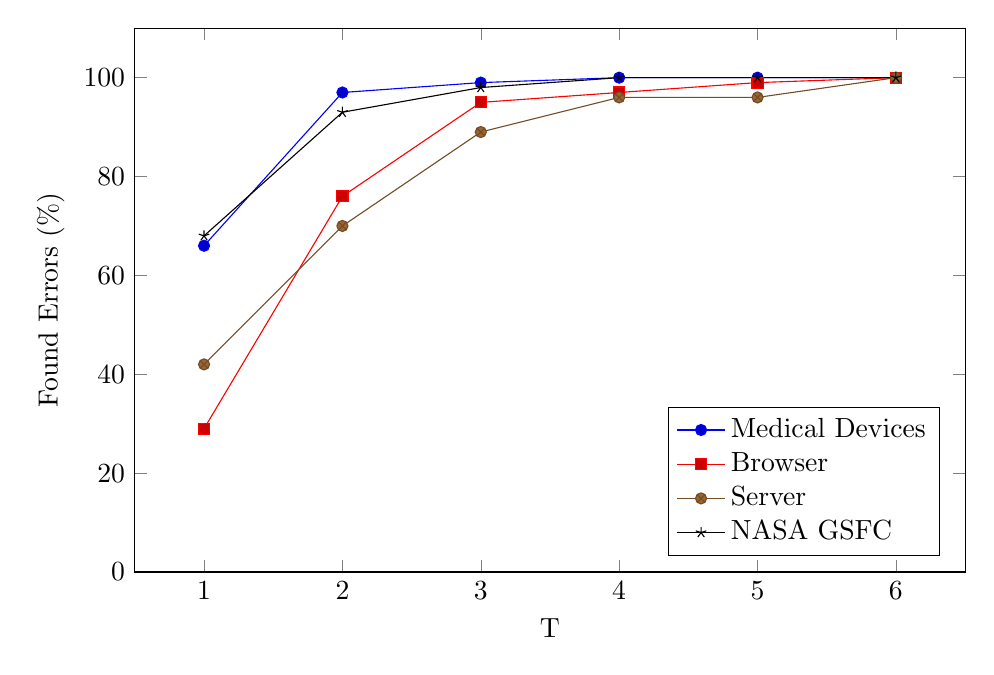
\begin{tikzpicture}
				\begin{axis}[
					width=\textwidth,height=.7\textwidth,
					%	ybar,
					ymin=0,ymax=110,
					xlabel=T,
					ylabel=Found Errors (\%),
					%	nodes near coords={\pgfmathprintnumber[precision=0]{\pgfplotspointmeta}},
					legend style={at={(0.97,0.03)},anchor=south east},
					legend cell align=left,
					]
					\addplot coordinates {(1,66) (2,97) (3,99) (4,100) (5,100) (6,100)};
					\addplot coordinates {(1,29) (2,76) (3,95) (4,97) (5,99) (6,100)};
					\addplot coordinates {(1,42) (2,70) (3,89) (4,96) (5,96) (6,100)};
					\addplot coordinates {(1,68) (2,93) (3,98) (4,100) (5,100) (6,100)};
					\legend{Medical Devices,Browser,Server,NASA GSFC}
				\end{axis}
			\end{tikzpicture}
		\end{exampletight}
		\begin{note}{Trade-Off}
			large t: high coverage (more effective)
			
			small t: low testing effort (more efficient)
		\end{note}
	\end{fancycolumns}
\end{frame}

\widexkcdframe{974} % salt 12s

%\begin{frame}{Einfache Heuristik für Pairwise Interaction Testing}
%	Greedy-Algorithmus: Wähle immer die Konfiguration als nächstes, die die meisten fehlenden Interaktionen abdeckt
%	\vspace{2mm}\pause
%	\begin{itemize}
	%		\item Erste Konfiguration frei wählbar (jede deckt am Anfang die gleiche Anzahl von Interaktionen ab: eine pro Paar)
	%		\item Stoppe wenn keine Interaktionen übrig
	%		\item Findet ggfs.\ nicht die kleinste Teilmenge an Konfigurationen
	%		\item Bessere Algorithmen wurden in den letzten Jahren vorgeschlagen (z.B. ICPL)
	%	\end{itemize}
%\end{frame}

% TODO introduce ICPL

\subsection{Combinatorial Interaction Testing in Practice}
\begin{frame}{Combinatorial Interaction Testing with ICPL\ \mytitlesource{\icpl}}
	\begin{fancycolumns}
		\begin{exampletight}{Assumption: All Features are Optional}
			\centering\pic[width=.66\textwidth]{productlines/optional-features}
		\end{exampletight}
		
		\begin{exampletight}{Number of Configurations in Pairwise Sample}
			\footnotesize\centering
			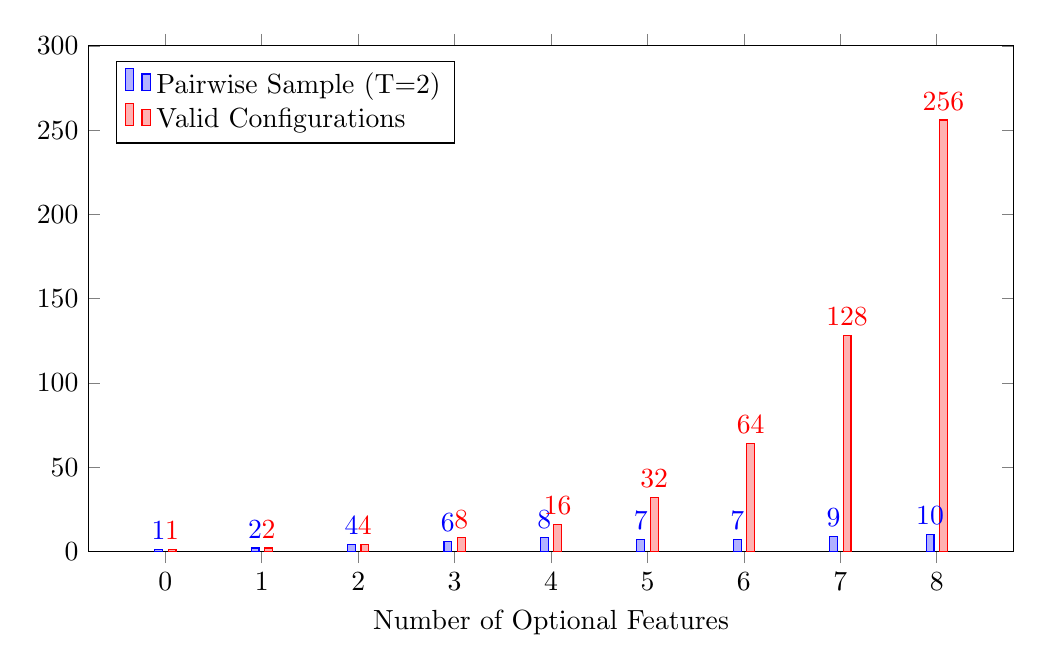
\begin{tikzpicture}
				\begin{axis}[
					width=1.1\textwidth,height=.66\textwidth,
					ybar,
					bar width=1mm,
					ymin=0,ymax=300,
					xlabel=Number of Optional Features,
					nodes near coords={\pgfmathprintnumber[precision=0]{\pgfplotspointmeta}},
					y label style={overlay},
					legend style={at={(0.03,0.97)},anchor=north west,fill=none},
					legend cell align=left,
					]
					\addplot coordinates {(0,1) (1,2) (2,4) (3,6) (4,8) (5,7) (6,7) (7,9) (8,10)};
					\addplot coordinates {(0,1) (1,2) (2,4) (3,8) (4,16) (5,32) (6,64) (7,128) (8,256)};
					\legend{Pairwise Sample (T=2),Valid Configurations}
				\end{axis}
			\end{tikzpicture}
		\end{exampletight}
		\nextcolumn
		\begin{exampletight}{Assumption: All Features are Optional}
			\centering\pic[width=.66\textwidth]{productlines/optional-features}
		\end{exampletight}
		
		\begin{exampletight}{Number of Configurations in T-Wise Sample}
			\footnotesize\centering
			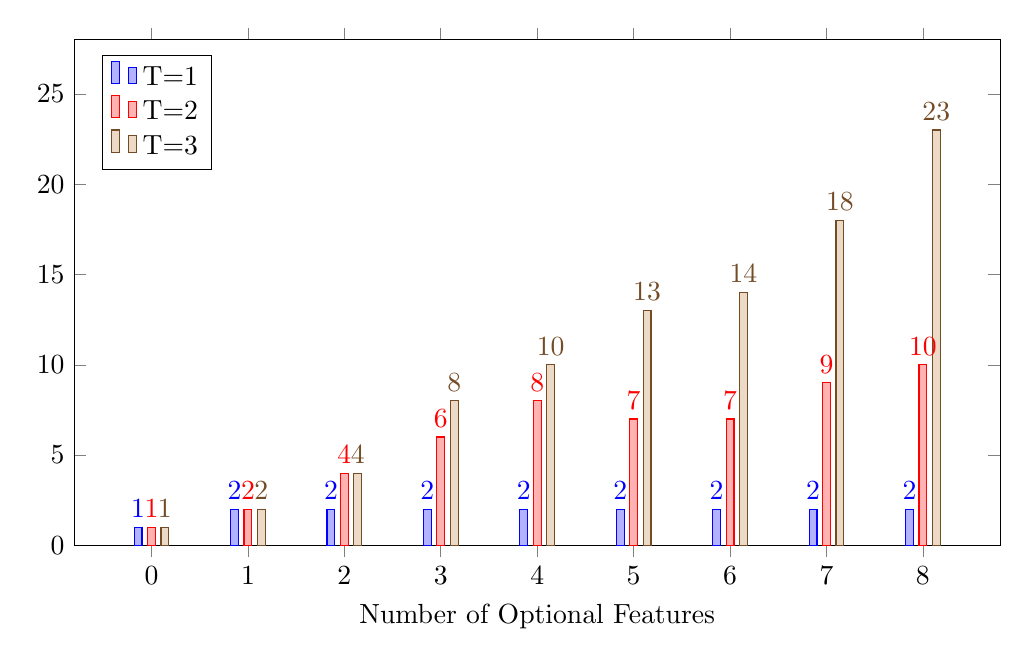
\begin{tikzpicture}
				\begin{axis}[
					width=1.1\textwidth,height=.66\textwidth,
					ybar,
					bar width=1mm,
					ymin=0,ymax=28,
					xlabel=Number of Optional Features,
					nodes near coords={\pgfmathprintnumber[precision=0]{\pgfplotspointmeta}},
					y label style={overlay},
					legend style={at={(0.03,0.97)},anchor=north west,fill=none},
					legend cell align=left,
					]
					\addplot coordinates {(0,1) (1,2) (2,2) (3,2) (4,2) (5,2) (6,2) (7,2) (8,2)};
					\addplot coordinates {(0,1) (1,2) (2,4) (3,6) (4,8) (5,7) (6,7) (7,9) (8,10)};
					\addplot coordinates {(0,1) (1,2) (2,4) (3,8) (4,10) (5,13) (6,14) (7,18) (8,23)};
					\legend{T=1,T=2,T=3}
				\end{axis}
			\end{tikzpicture}
		\end{exampletight}
	\end{fancycolumns}
\end{frame}

%\begin{frame}{Recap: Feature Model of the Linux Kernel}
%	\slideLinuxFeatureModel
%\end{frame}

\begin{frame}{Pairwise Interaction Testing in Practice\ \mytitlesource{\icpl}}
	\begin{fancycolumns}
		\begin{exampletight}{Time in Minutes to Compute Sample}
			\footnotesize\centering
			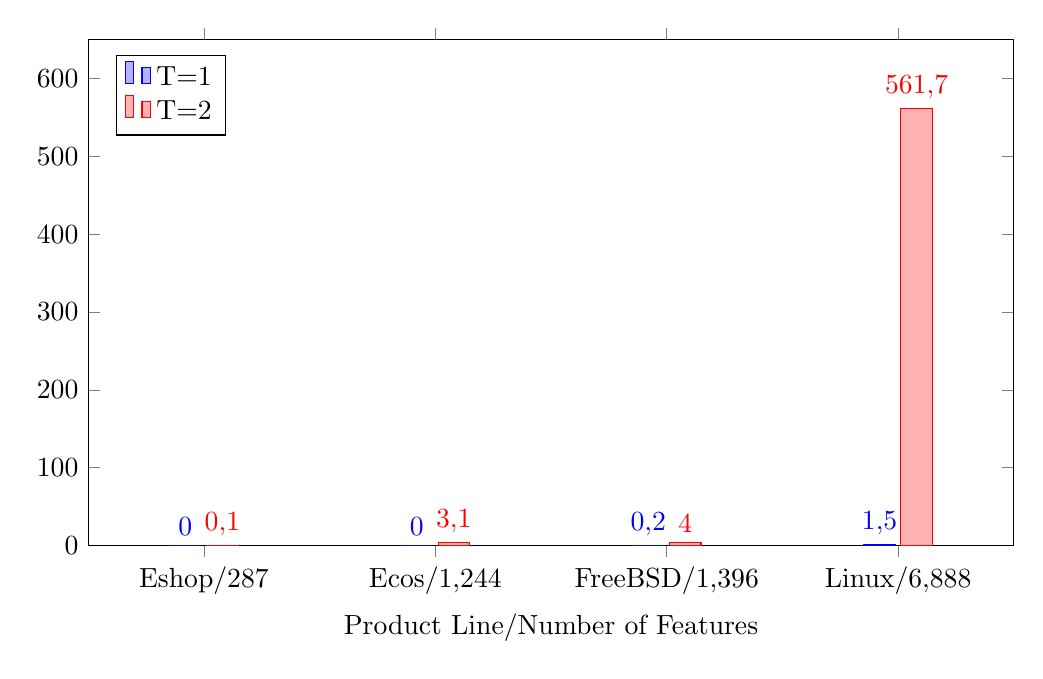
\begin{tikzpicture}
				\begin{axis}[
					/pgf/number format/.cd,use comma,1000 sep={.},
					width=1.1\textwidth,height=.66\textwidth,
					ybar,
					bar width=4mm,
					ymin=0,ymax=650,
					xmin=-.5,xmax=3.5,
					xlabel=Product Line/Number of Features,
					xtick={0,1,2,3},
					xticklabels={Eshop/287,{Ecos/1,244},{FreeBSD/1,396},{Linux/6,888}},
					nodes near coords={\pgfmathprintnumber[precision=1,fixed]{\pgfplotspointmeta}},
					y label style={overlay},
					legend style={at={(0.03,0.97)},anchor=north west,fill=none},
					legend cell align=left,
					]
					\addplot coordinates {(0,0) (1,0) (2,.2) (3,1.5)};
					\addplot coordinates {(0,.1) (1,3.1) (2,4.0) (3,561.7)};
					%	\addplot coordinates {(0,7.6) };
					\legend{T=1,T=2,T=3}
				\end{axis}
			\end{tikzpicture}
		\end{exampletight}
		\begin{example}{}
			\begin{itemize}
				\item about 9h for Linux
				\item 480 configuration in pairwise sample
			\end{itemize}
		\end{example}
		\nextcolumn
		\begin{exampletight}{Number of Configurations in Sample}
			\footnotesize\centering
			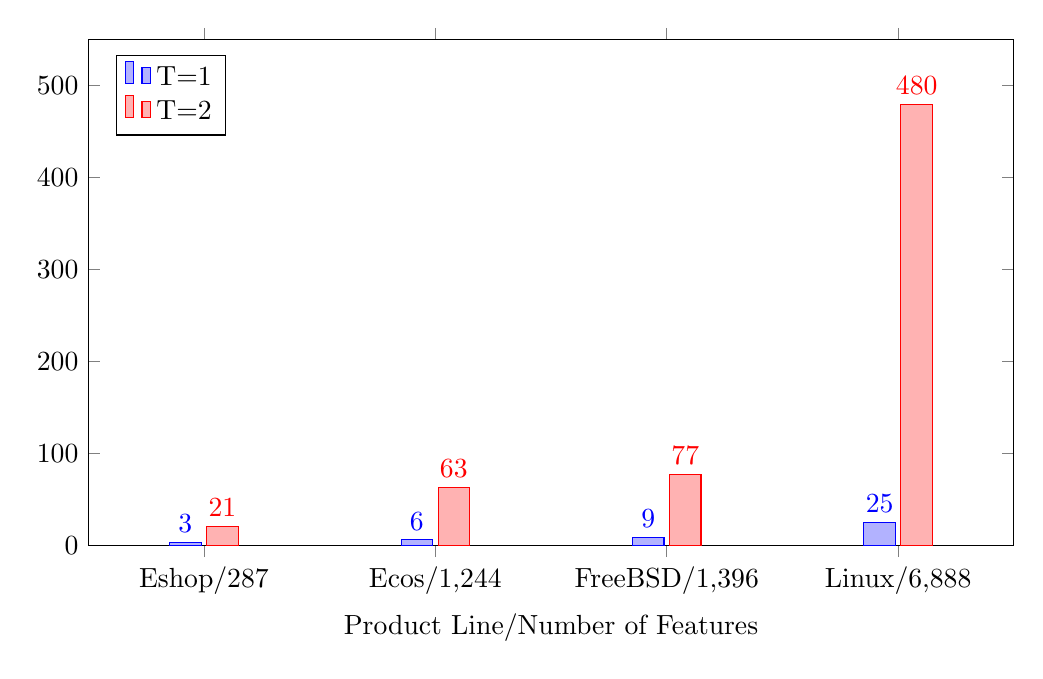
\begin{tikzpicture}
				\begin{axis}[
					/pgf/number format/.cd,use comma,1000 sep={.},
					width=1.1\textwidth,height=.66\textwidth,
					ybar,
					bar width=4mm,
					ymin=0,ymax=550,
					xmin=-.5,xmax=3.5,
					xlabel=Product Line/Number of Features,
					xtick={0,1,2,3},
					xticklabels={Eshop/287,{Ecos/1,244},{FreeBSD/1,396},{Linux/6,888}},
					nodes near coords={\pgfmathprintnumber[precision=0]{\pgfplotspointmeta}},
					y label style={overlay},
					legend style={at={(0.03,0.97)},anchor=north west,fill=none},
					legend cell align=left,
					]
					\addplot coordinates {(0,3) (1,6) (2,9) (3,25)};
					\addplot coordinates {(0,21) (1,63) (2,77) (3,480)};
					%	\addplot coordinates {(0,108) };
					\legend{T=1,T=2,T=3}
				\end{axis}
			\end{tikzpicture}
		\end{exampletight}
		\begin{example}{}
			\begin{itemize}
				\item Linux kernel v2.6.28.6 (February 2009)
				\item 6,888 features, 187,193 clauses in conjunctive normal form
			\end{itemize}
		\end{example}
	\end{fancycolumns}
\end{frame}

% TODO how Linux is developed: patches on mailing list, only considered if not rejected by CI, what happens in CI

% TODO variant reduction, prevent the explosion. marketing wants them all. engineering and quality assurance too expensive.

\begin{frame}{Number of Features in Linux\ \mytitlesource{\href{https://www4.cs.fau.de/Ausarbeitung/MA-I4-2015-04-Hengelein.pdf}{Hengelein 2015}}}
	\begin{fancycolumns}[widths={70}]
		\begin{exampletight}{{2005--2015: Number of Features Tripled}}
			\pic[width=\linewidth]{productlines/linux-features}
		\end{exampletight}
	\end{fancycolumns}
\end{frame}

\subsection{Wisdom on Features}
\begin{frame}{Choose Features Wisely}
	\begin{fancycolumns}
		\begin{exampletight}{John Ferguson Smart (2017)}
			\centering\picDark[width=.98\linewidth,angle=2,trim=0 0 5 0,clip]{productlines/unnecessary-features}
		\end{exampletight}
		% 
		\nextcolumn
		\centering\pic[width=.47\linewidth,trim=0 0 0 0,clip]{people/john-carmack}
		\vspace{-7mm}
		
		\begin{note}{John Carmack (born 1970) \mysource{\href{https://www.ics.uci.edu/~pattis/quotations.html\#C}{uci.edu}}}
			\mycite{The important point is that the cost of adding a feature isn't just the time it takes to code it. The cost also includes the addition of an obstacle to future expansion. %Sure, any given feature list can be implemented, given enough coding time. But in addition to coming out late, you will usually wind up with a codebase that is so fragile that new ideas that should be dead-simple wind up taking longer and longer to work into the tangled existing web. 
				[...] The trick is to pick the features that don't fight each other.}
		\end{note}
		% video game developer, co-founder of a video game company
	\end{fancycolumns}
\end{frame}

\lessonslearned{
	\item All configurations? one configuration? feature interactions!
	\item Combinatorial interaction testing:\\pairwise and t-wise
	\item Trade-off between:\\sample coverage (effectiveness) vs\\ sample size (testing efficiency) vs\\ time to compute sample (sampling efficiency)
	\item Next: Why is automotive software so challenging?
}{
	\item \icpl --- famous ICPL algorithm
	\item \href{https://dl.acm.org/doi/10.1145/3712193}{Krupke~et~al.} --- first algorithm that can compute the smallest sample
}{
	Quiz in \StudIP

	~
	
	\centering\fancyqr{color=black,height=30mm}{https://studip.tu-braunschweig.de/dispatch.php/course/courseware/courseware/18333?cid=635f5186b364a369979d0f45ab2ace1d\#/structural\_element/421054}
}

%\faq{
%	\item
%}{
%	\item
%}{
%	\item
%}

\input{../se1/template/footer}

% TODO L12 Automotive Software

\ifuniversity{tubs}{\date{July 7, 2025}}

\author{Thomas Thüm}
\lecture{Automotive Software}{automotive}

\xkcdframe{2948}

\section{Part 1}
%\input{content/a-}
\lessonslearned{
	\item ?
	\item Next: ?
}{
	\item \sommerville\mychapter{?} 
}{
	\begin{enumerate}
		\item<+-> Form groups of 2--3 students
		\item<+-> ?
	\end{enumerate}
}

\section{Part 2}
%\input{content/b-}
\lessonslearned{
	\item ?
	\item Next: ?
}{
	\item \sommerville\mychapter{?} 
}{
	\begin{enumerate}
		\item<+-> Form groups of 2--3 students
		\item<+-> ?
	\end{enumerate}
}

\section{Part 3}
%\input{content/c-}
\lessonslearned{
	\item ?
	\item Next: ?
}{
	\item \sommerville\mychapter{?} 
}{
	\begin{enumerate}
		\item<+-> Form groups of 2--3 students
		\item<+-> ?
	\end{enumerate}
}

%\faq{
%	\item
%}{
%	\item
%}{
%	\item
%}

\input{../se1/template/footer}
